% Look Sebastian fisher (a play on regular expression) 
%   Really goes all the way 

% Student Sven is working on a Robot programming DSL supervised by Prof. Kurt. 
% Sven is beginner Haskeller
% Kurt is knowledgible (experienced)

% Introduction (Presents problem) 
%  Robot language operations. 
%  Robot exists that run programs in a simple language.
%  want to run code in robot. 
%  Haskell DSL and Do notation 
%  Compilation necessary.  

% Student has Haskell School of expression 
%   But need reifyable robot programs (evaluation not enough) 

% Show example program early 
%   Sven is a good student and early expresses an example program in his thought 
%   out API.
% 

% How to be able to use Do notation 
%  Adds Return and Bind naively to data structure. 

% Student brings --CODE SNIPPET-- to Prof. Kurt.

% Now the problem, how can this work? 
%  Prof. is familiar with Gills blog post. 

% Student brings --CODE SNIPPET-- (the compiler) to Prof. 


% Surprise 
% Work on generalisations  and make the compositionality explicit
% 

% What about the monad laws ? 
%  Prof. asks student to verify that Monad laws hold.


\section{Introduction}
\studname{} is a computer science student working in a project involving programming 
robots in a low level imperative language. However, \studname{} has a budding 
interest in functional programming using Haskell and has read ``The Haskell 
school of expression'' \cite{HUDAK}. Naturally he gets the idea to implement 
a language for robot control embedded in Haskell. \studname{} realise that the 
capabilities of their robot hardware is very similar to those of the 
robots that Hudak evaluates graphically in a grid world. There is however 
a very important difference; the embedded language needs to be compiled into 
some form that is understood by the robot. 
%\studname{} in a computer science student with a budding interest in functional 
%programming using Haskell. \studname{} is developing  
%an embedded domain specific language (EDSL) for robot control. Inspired 
%by the book ``the Haskell school of expression'' \cite{HUDAK} but instead of 
%evaluating his robot EDSL, \studname{} wants to compile the language to a form 
%he can run on actual robot hardware. 
%with 
%different motivations, \studname{} wants compile his EDSL for actual physical robots, 
%he sets out. 

Guided by the capabilities of the target robot, \studname{} designs an API for 
robot programming. Amongst the capabilities of the robot are operations 
such as {\em move} that steps the robot forward and {\em turn} left and right. 
The robot also has a forward facing {\tt sensor} with which it can query the 
world and also the capabilities to execute program loops and conditionals. 

The API that \studname{} designs is simple: 

%\begin{figure} 
\begin{small}
\begin{verbatim} 
move :: Program () 
turnLeft :: Program () 
turnRight :: Program ()
sensor :: Program Bool 
cond :: Bool -> Program () -> Program () -> Program () 
while :: Program Bool -> Program () -> Program () 
\end{verbatim}
\end{small} 
%\label{fig:interface} 
%\caption{Proposed set of basic robot operations}
%\end{figure}  

Now, \studname{} wants to express robot programs using the Haskell {\em do} 
notation. The motivation behind this is the imperative look and feel 
of the operations he identified and the potential to use all the control structures 
in the {\em Control.Monad} library. For this, a {\tt Monad} instance is needed. 

%\begin{minipage}[]{\linewidth}
\vspace{5mm}

\fbox{%
\parbox{0.8\linewidth}{What \studname{} does not know at this time is that he has stumbled over the 
problem of {\em Monad reification}. Monad reification is the observing of the shape of the computation and this is necessary in order to compile to some low level representation.}
}
%\end{minipage}

\subsection{Example programs}
After listing the desired basic operations of the language, \studname{} tries to write 
a few very simple example programs.
%experiments 
%with what some of these robot controlling programs could look like once his 
%EDSL is finished. 

The first program written is one called sMove, that implements a safe move 
operation. This operation can be executed by the robot even though it is facing 
an obstacle without risk of harming robot or obstacle. 
%.It feels like a good idea to \studname{} to check the sensor before trying to 
%move the robot forward. Otherwise something in either the world or the 
%robot might suffer damage. 

\begin{small} 
\begin{verbatim}
sMove :: Program () 
sMove = do 
  s <- sensor 
  cond s turnRight move 
\end{verbatim}
\end{small}  

The second program he writes moves the robot forward until it stands directly 
in front of an obstacle such as a wall. 

\begin{small} 
\begin{verbatim}
moveToWall :: Program () 
moveToWall = while ((liftM not) sensor) move
\end{verbatim}
\end{small}  

Based on these examples, \studname{} is quite satisfied with the design of his
language and turns to implementing it.

\subsection{Implementation and data structures} 

Enthused by the prospect of compiling these programs to the target language and 
seeing some robot action, \studname{} goes to work on the data structures. 

Since an abstract syntax representation of the robot programs is desired, \studname{} 
realises that the booleans of some of the operations needs to be replaced by 
boolean typed expressions. 

\begin{small} 
\begin{verbatim}
data BoolE = Lit Bool
           | Var String
           | (:||:) BoolE BoolE
           | (:&&:)  BoolE BoolE
           | Not BoolE  
\end{verbatim} 
\end{small}  

following this, the  operations that should go into the {\tt Program} data type 
feels straightforward.

\begin{small} 
\begin{verbatim}
data Program a where 
  Move :: Program () 
  TurnLeft :: Program () 
  TurnRight :: Program () 
  Sensor :: Program BoolE
  Cond :: BoolE -> Program () -> Program () 
  While :: Program BoolE -> Program () -> Program () 
\end{verbatim} 
\end{small} 

\studname{} continues by naively adding constructors for {\tt Return} and 
{\tt Bind} to the {\tt Program a} data type.   

\begin{small} 
\begin{verbatim}
data Program a where 
  ...
  Return :: a -> Program a 
  Bind :: Program a -> (a -> Program b) -> Program b 
\end{verbatim} 
\end{small} 

Then he writes down the {\tt Monad} instance.
 
\begin{small} 
\begin{verbatim}
instance Monad Program where 
  return = Return 
  (>>=)  = Bind 
\end{verbatim} 
\end{small} 

Proud of his accomplishments, \studname{} sends his Haskell module in an email to Prof. \docname{}.
\studname{} knows that \docname{} is teaching an introductory Haskell course and should be 
able to provide feedback.



\section{Problem statement} 
\emph{Meanwhile in Professor \docname{}'s Office}\newline \newline

\noindent Prof. \docname{} notices an email from \studname{} in his inbox and opens it. 

\vspace{5mm} 

\noindent\colorbox{light-gray}{
\begin{minipage}[]{0.9\linewidth}
\noindent 
Dear Professor \docname{}
\newline \newline
\noindent I am CS student working in a robot control project. Usually, we 
program our robots in C but I have developed an interest in Haskell 
programming and thought it'd be natural to try implementing an EDSL. 
I know you teach an FP course and thought id ask for your input. 
Atached to this mail is a file containing an outline of the data types I 
want to use. Does this look sensible to you? \newline \newline

\noindent Thank you \newline
\noindent \studname{}
\end{minipage} 
}

%I have progressed some towards a robot programming language. Attached 
%to this mail is a first sketch of a {\tt Program a} data type for robot 
%programs.
\vspace{5mm}

Prof. \docname{} opens the attachment and takes a look at the data type. He 
particularly notices the constructors {\tt Return} and {\tt Bind} and the 
{\tt Monad} instance. He shakes his head at \studname{}'s naivety and writes an 
email back:

\vspace{5mm}

\noindent\colorbox{light-gray}{
\begin{minipage}[]{0.9\linewidth}
\noindent 
Hello \studname{}
\newline \newline
\noindent I'm afraid your implementation of the monadic primitives can never 
work. The constructor {\tt Return} can take any arbitrary value which has 
nothing to do with the language you're designing. These values may be 
strings, binary trees of higher order functions from zygomorphisms to 
histomorphisms. The same problem goes for {\tt Bind}, it has to be able 
to handle arbitrary values. It cannot possibly work! This is a very 
difficult problem and such a naive solution is bound to fail. 

\noindent For hints towards a solution to this I suggest that you follow 
this \underline{link} \cite{GillBlog}. Another idea is that you refer 
to the article ``Generic monadic constructs for embedded languages'' 
\cite{Generic}. \newline \newline 

\noindent Prof. \docname{} \newline
\noindent Dept. of Computer Science and Engineering \newline
\noindent Chalmers University of Technology 
\end{minipage} 
}

\vspace{5mm}


\section{Implementation continues}
\emph{Back to \studname{}'s implementation efforts} \newline \newline

\noindent While waiting for feedback from \docname{}, \studname{} has carried on trying to implement
a compiler for his language. 

When \docname{}'s email does arrive, \studname{} is confused. He feels he has already managed 
to compile the {\tt Program a} data type into a representation closer to that 
which is executed by the robot hardware. 

He writes an apprehensive email back to Prof. \docname{}. 

\vspace{5mm}

\noindent\colorbox{light-gray}{
\begin{minipage}[]{0.9\linewidth}
\noindent 
Hello Prof. \docname{} 
\newline \newline
\noindent Thanks for your feedback. But I think it does work! attached 
to this email (Compiler.hs) you find my attempt at compiling the 
{\tt Program a} into a representation closer to that which is executed 
by our robots. \newline \newline

\noindent \studname{} 
\end{minipage} 
}

\vspace{5mm}


\section{Compilation of the monadic robot EDSL} 
\emph{\docname{} receives \studname{}'s latest email}\newline \newline 

\noindent \docname{} looks through the {\tt Compiler} module and finds a data type describing
a first order representation of the robot language.

\begin{small} 
\begin{verbatim}
data Prg = PMove          
         | PTurnRight
         | PTurnLeft
         | PSensor Var    
         | PCond BoolE Prg Prg
         | PWhile Var Prg Prg 
         | PSeq Prg Prg
         | PSkip       
         | PAssign Var BoolE
\end{verbatim}
\end{small}

From the {\tt Prg} data type, \docname{} presumes that the {\tt PSeq} constructor 
will replace occurences of {\tt Bind} and that the variable binding of the 
{\tt Sensor} construct is reified using {\tt PAssign}. The conclusion is
that the representation looks sensible but he is very interested in seeing 
the {\tt Program a -> Prg} transformation. 

\begin{small} 
\begin{verbatim}
compile :: Program a -> Prg
compile prg = snd $ compile' s prg 
  where 
    s = unsafePerformIO $ newEnumSupply
    
compile' :: Supply Int -> Program a -> (a, Prg) 
compile' s Move = ((),PMove)
compile' s TurnRight = ((),PTurnRight)
compile' s TurnLeft  = ((),PTurnLeft)
compile' s Sensor    = (Var nom,PSensor nom)
  where
    v = supplyValue s
    nom = "v" ++ show v 
compile' s (Cond b p1 p2) = ((), PCond b p1' p2') 
  where
    (s1,s2) = split2 s
    (a1,p1') = compile' s1 p1
    (a2,p2') = compile' s2 p2 
compile' s (While wp prg) = ((),PWhile nom nwp prg') 
  where
    (s1,s2,s3) = split3 s
    (b,wp') = compile' s1 wp
    (c,prg') = compile' s2 prg 
    nom  = "v" ++ (show $ supplyValue s3)
    nwp = (wp' `PSeq` PAssign nom b) 
compile' s (Return a) = (a,PSkip)
compile' s (Bind pa f) = (b, prg1 `PSeq` prg2) 
  where
    (s1,s2) = split2 s
    (a,prg1) = compile' s1 pa
    (b,prg2) = compile' s2 (f a) 
\end{verbatim}
\end{small}

\docname{} studies the code in disbelief but saves the module to his harddrive 
and tries it out on some examples. The code does indeed seem to work and 
\docname{}'s disbelief is replaced with enthusiasm, this appears to be a simple 
and conveniant way to reify monads. what's more it does so in a 
compositional way. The compilation of the {\tt Return} and {\tt Bind} cases 
are completly independent of any other construct of the language. 

\docname{} sends an email to \studname{}, inviting him to a meeting. 

\section{Related Work} 
\emph{Meeting in \docname{}'s office} \newline 

%TODO Here I want to cast light on more related work 
%and have \docname{} and \studname{} compare their approach to some of the existing ones. 
%also they should start sketching out the Idea of using {\tt CompData} instead 
%of a la carte for showing the compositionality. 

%\begin{minipage}[]{\linewidth}
\begin{dialogue} 

\speak{\docname{}} Hello, come in. 

\speak{\studname{}} Thanks. 

\speak{\docname{}} So, about this robot language! you gave me a bit of a 
surprise there. I was entirely sure that what you did was impossible. 

\speak{\studname{}} Oh, But I just did the first thing that came to mind. 
There was no deep thought behind it. 

\speak{\docname{}} The problem is \direct{\docname{} approaches his whiteboard}
 when you try to reify the bind constructor of your representation..
\end{dialogue} 


%\mbox{ 
\begin{small}
\begin{Verbatim}[commandchars=\\\{\}] 
Bind :: Program a -> \underline{(a -> Program b)} -> Program b 
\end{Verbatim}
\end{small}
%}


\begin{dialogue}
\speak{\docname{}} you need to come up with an element of type a to pass to the 
function. 

\speak{\studname{}} I didn't realise it was problem. 

\speak{\docname{}} But it is. I have never seen a solution as naive as yours 
though and was quite surprised that it works. 

\speak{\docname{}} For example, in this paper \cite{Generic}, the authors use 
a continuation monad to be able to reify the monadic constructs of their 
language

\end{dialogue}
\emph{Have \docname{} outline the continuation monad approach on the whiteboard}

%\emph{Maybe here kurt can show related work and explain why these related
%approaches exist\cite{GillBlog}
%\cite{Farmer}
%\cite{Generic}
%\cite{Wouter}
%\cite{CompData}
%\cite{Compile} 
%\cite{MonadReader15}}

\begin{dialogue}
\speak{\docname{}} Your solution is that you are careful about the return types 
of other operations in your language. They are either of unit type or some 
in itself reifyable expression type. \direct{\docname{} scribbles on  his whiteboard}

\end {dialogue} 

\begin{small}
\begin{Verbatim}[commandchars=\\\{\}] 
Move :: Program \underline{()}
  
Sensor :: Program \underline{BoolE}
\end{Verbatim}
\end{small}

\emph{lots more text here} 

\begin{dialogue}

\speak{\docname{}} About compositionality, I think that we can make this explicit 
by using an approach based on \cite{Wouter} or \cite{CompData}.

\speak{\docname{}}  Bye!  
\end{dialogue}
%\end{minipage}


\section{Execution of the compiled representation} 
\emph{The discussion turns to practical}\newline \newline 
\FloatBarrier

%\begin{minipage}[]{\linewidth}
\begin{dialogue}

\speak{\docname{}} Let us see if we can implement some more interesting 
example programs in your language. Can you do spiral ? 

\speak{\studname{}} No. Infinite programs are ruled out by my compilation 
function. 

\speak{\docname{}} It is true that your compilation function rules out 
infinite programs but that is necessary to rule out such programs anyway 
if you want them to compile for our robot hardware. 
\speak{\docname{}} Write a spiralIn program with a well defined termination 
condition. 

\direct{\studname{} opens his laptop and starts hacking..} 
\end {dialogue} 
% \end{minipage}

\begin{small}
\begin{verbatim}
spiralIn :: Int -> Program () 
spiralIn 0 = return () 
spiralIn n = do
  replicateM_ 2 $ do
    replicateM_ n move
    turnLeft
  spiralIn (n-1) 
\end{verbatim}
\end{small}

% \begin{minipage}[]{\linewidth}
\begin{dialogue} 

\speak{\docname{}} yes. That should work. Do we have any way to verify this 
program. 

\speak{\studname{}} We can run it through the graphical simulator! 

\speak{\docname{}} Show me!

\end{dialogue}  

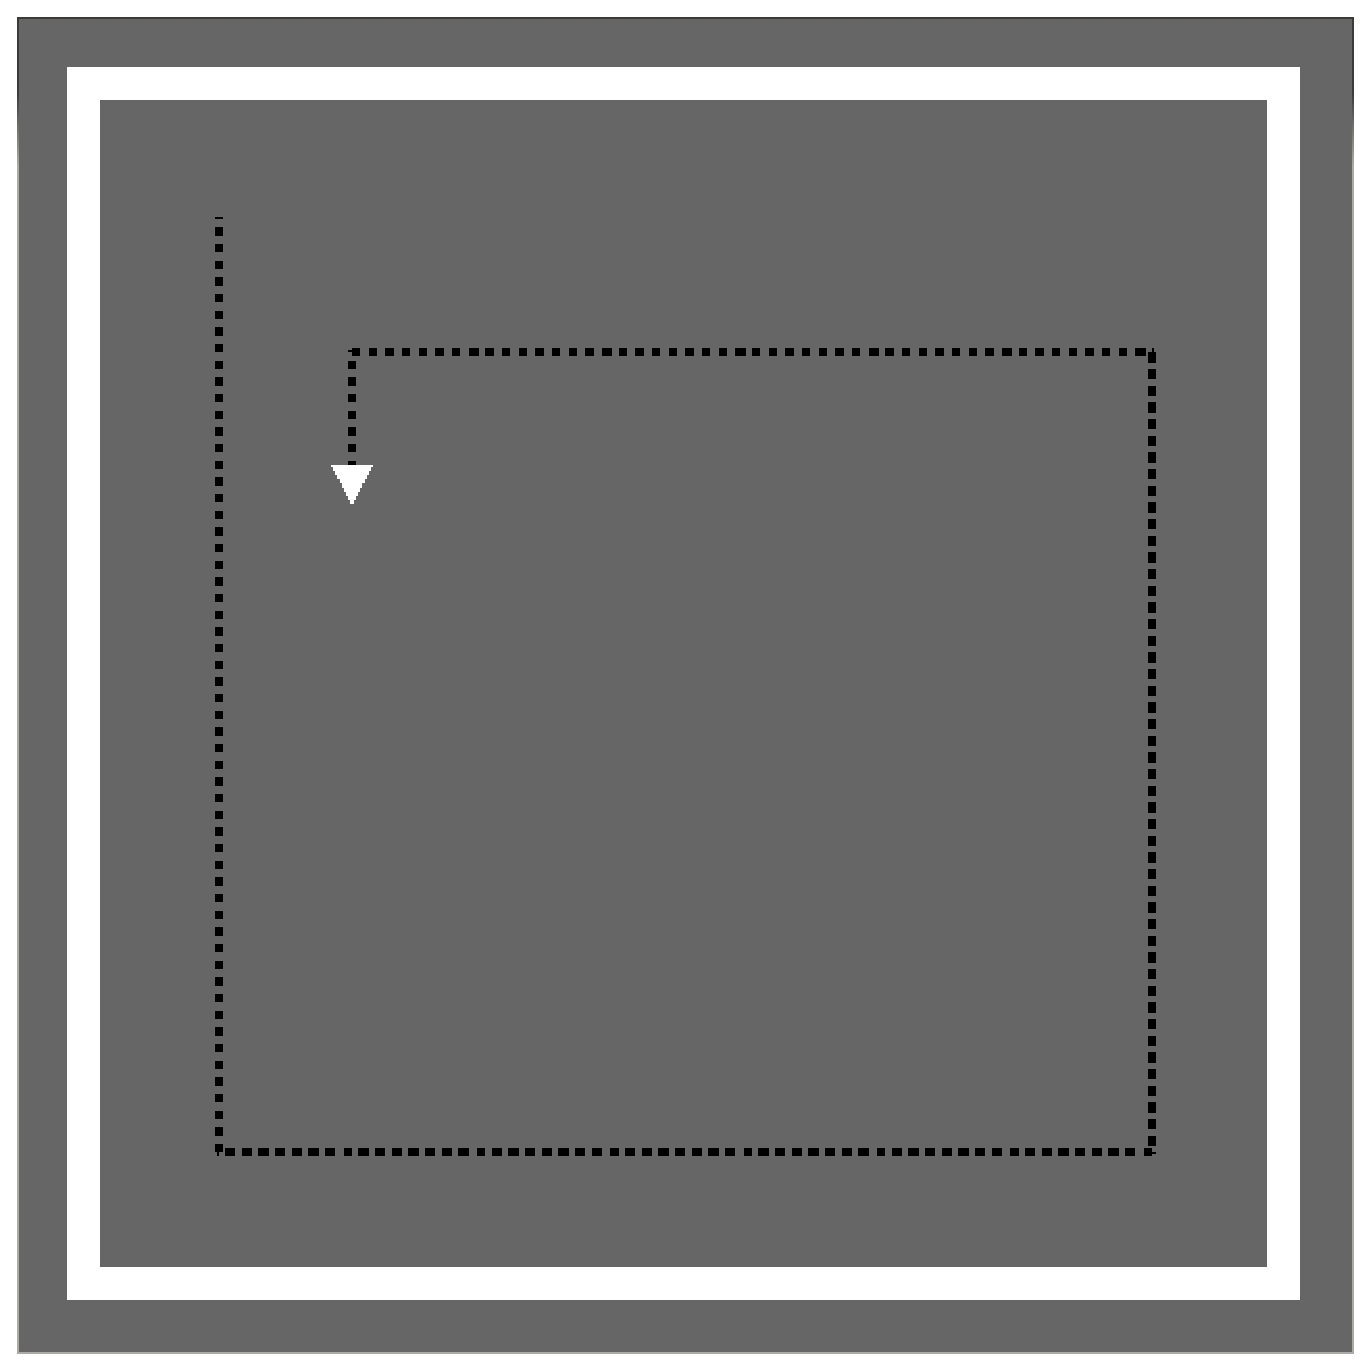
\includegraphics[width=.49\linewidth]{./spiral1}
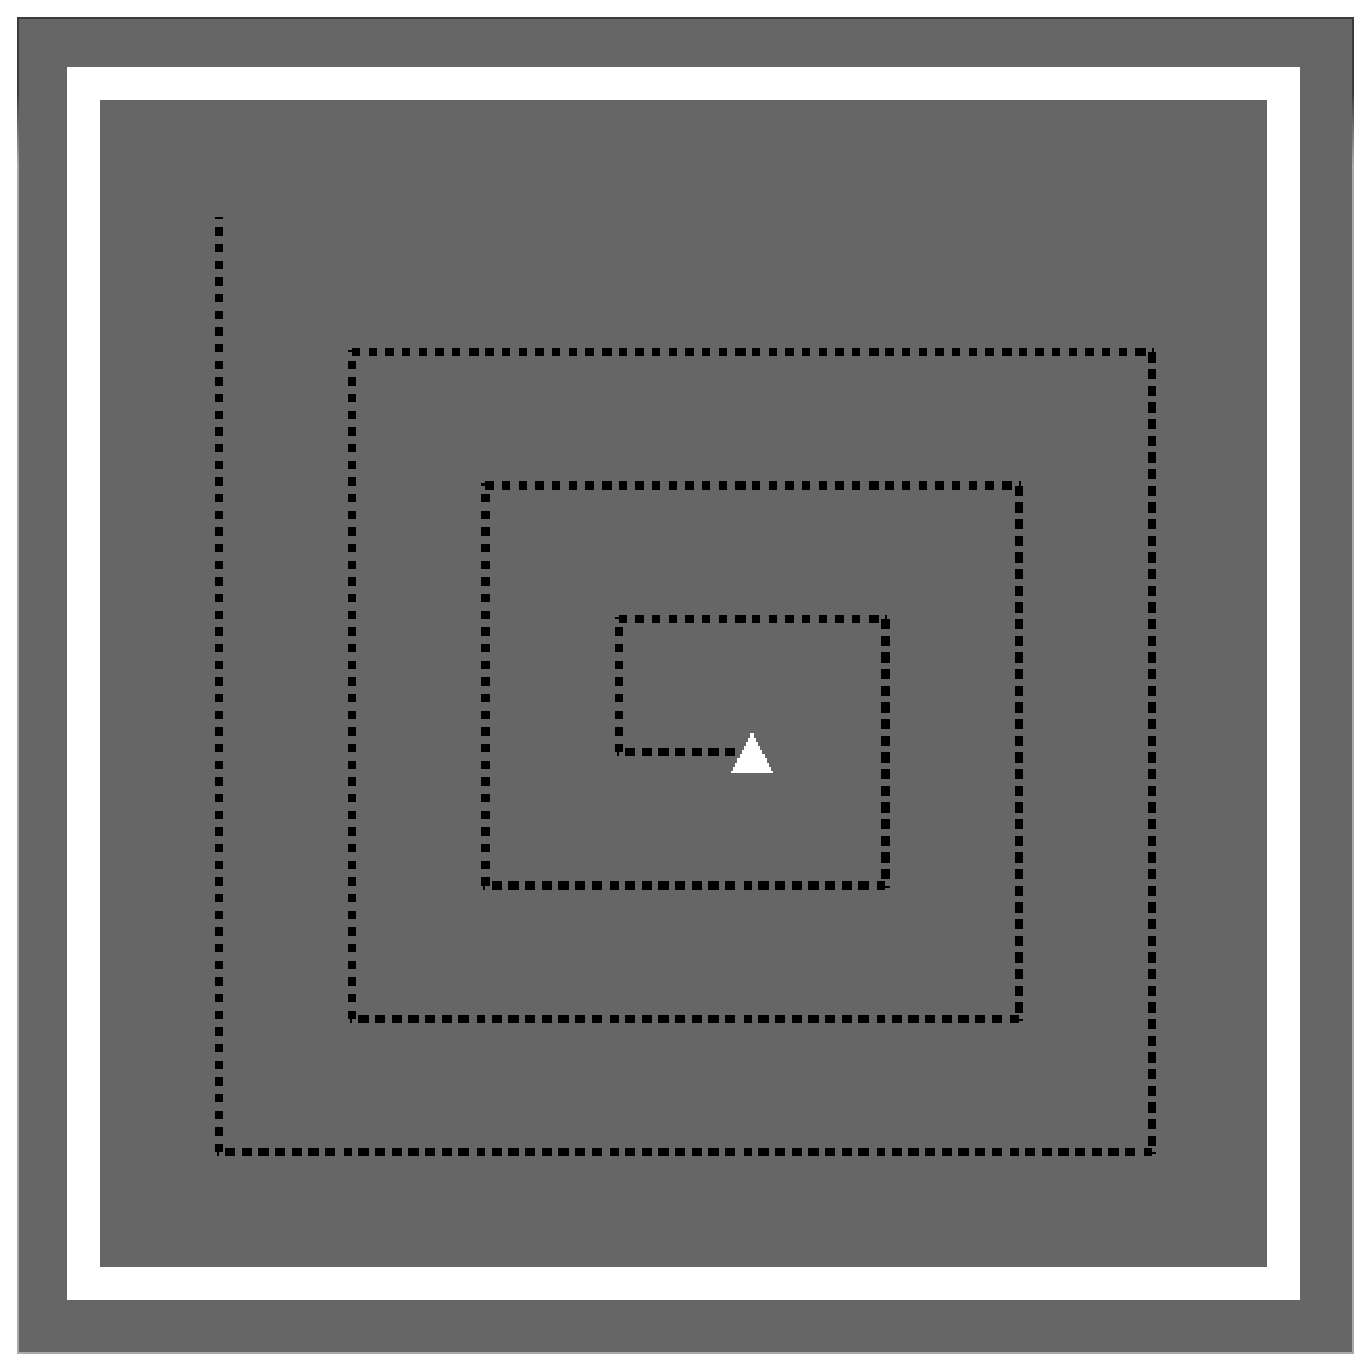
\includegraphics[width=.49\linewidth]{./spiral2}

\begin{dialogue} 

\speak{\docname{}} Nice! 

\speak{\docname{}} Now, let us try something more advanced. Can you program 
the robot to always keep a wall on his left hand side? 

\end{dialogue}  

\begin{small}
\begin{verbatim} 
followWall :: Program () 
followWall = do
  while (return true) $ do
    b <- checkLeft
    cond b sMove (turnLeft >> move) 
\end{verbatim}
\end{small}

\begin{dialogue} 
\speak{\docname{}} Yes. that looks about right. Let us see it. 
\end{dialogue}

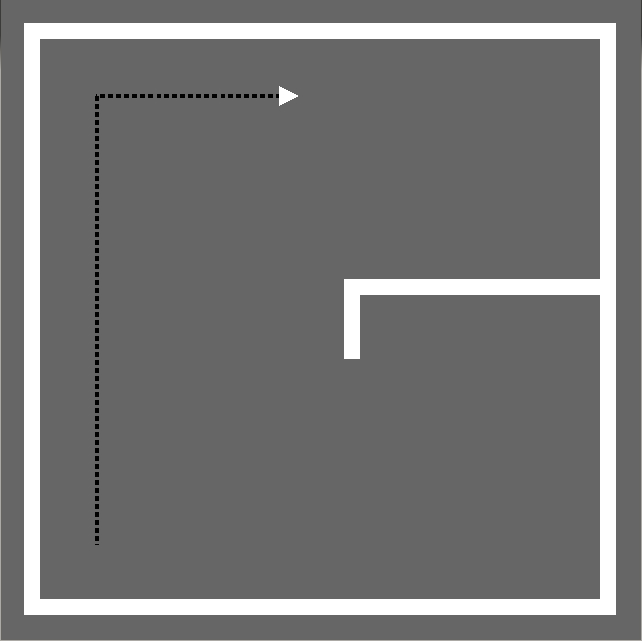
\includegraphics[width=.49\linewidth]{./wall1}
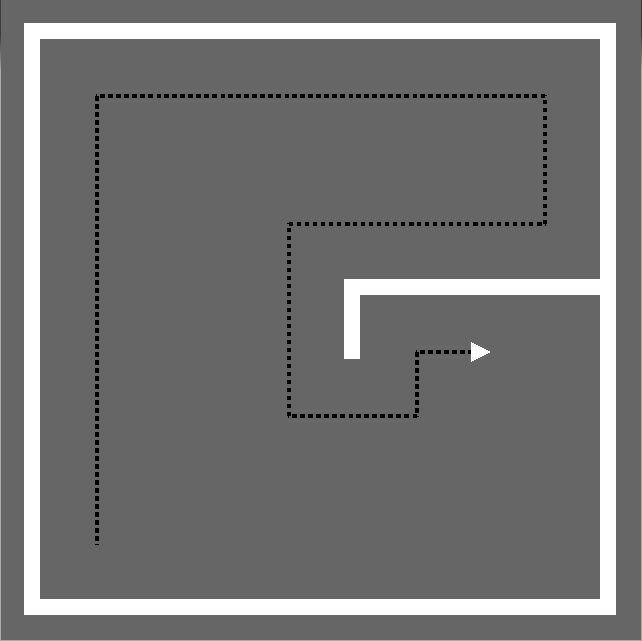
\includegraphics[width=.49\linewidth]{./wall2}

%\end{minipage}



%figure~\ref{fig:spiral}, shows the output generated from running the 
 %{\tt spiralIn} program.

%\studname{} feels motivated to try writing some program that shows a little bit more
%intelligence in the robot. A small program that makes sensible decisions based
%on the sensor information is implemented. 




%\begin{figure}
%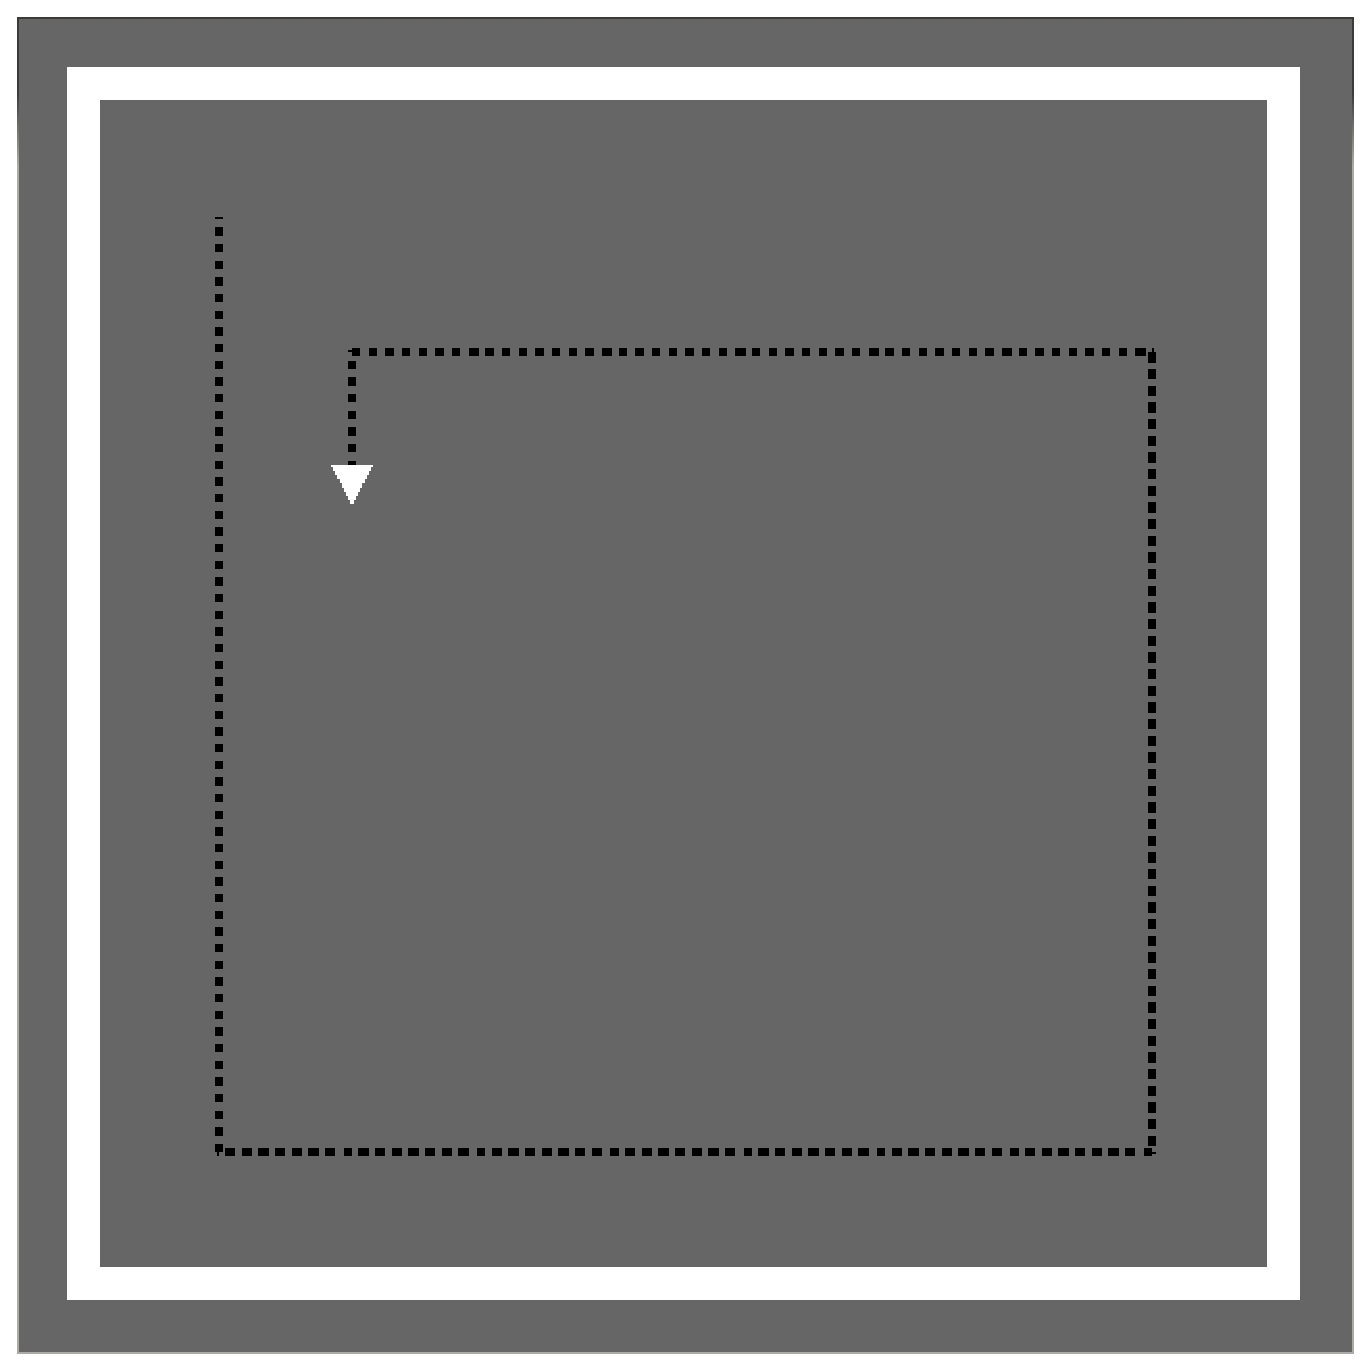
\includegraphics[width=.49\linewidth]{./spiral1}
%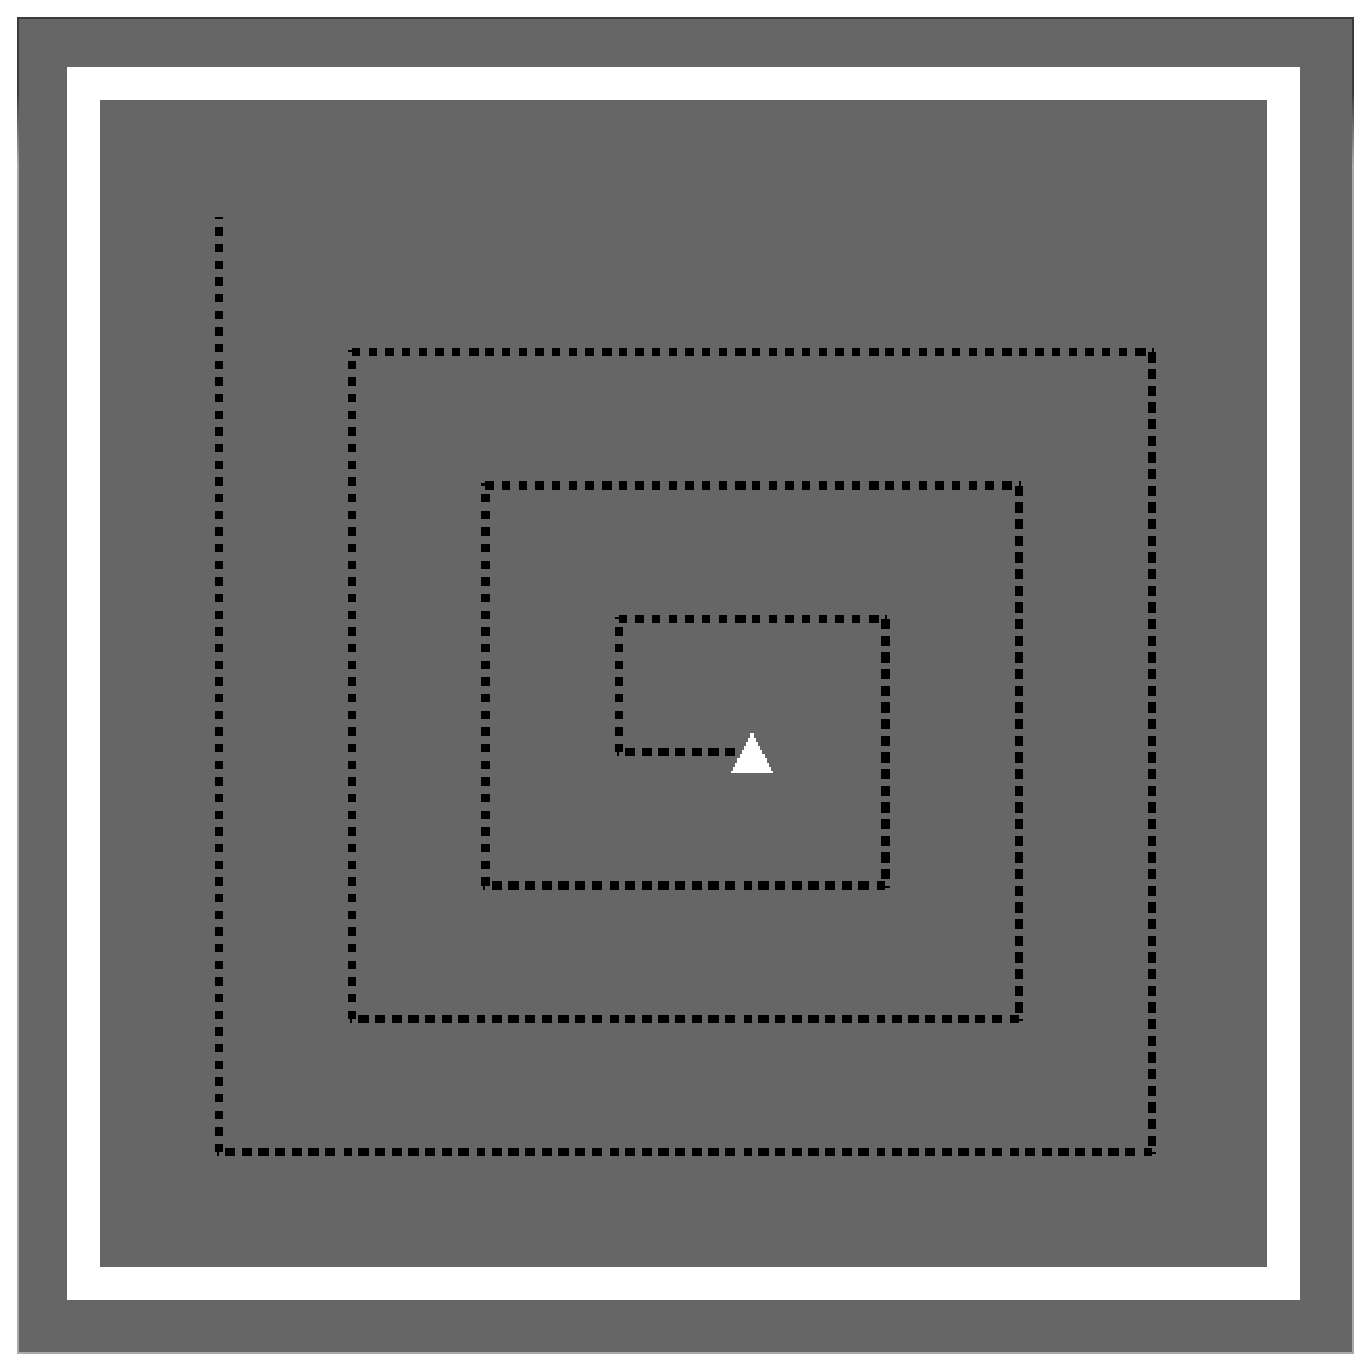
\includegraphics[width=.49\linewidth]{./spiral2}
%\caption{Images generated by our robot simulator using the {\tt spiral} program.An important detail is that the robot simulator does not evaluate the Monadic program but rather executes a compiled first order representation of that program.}
%\label{fig:spiral}
%\end{figure}


%\begin{figure}
%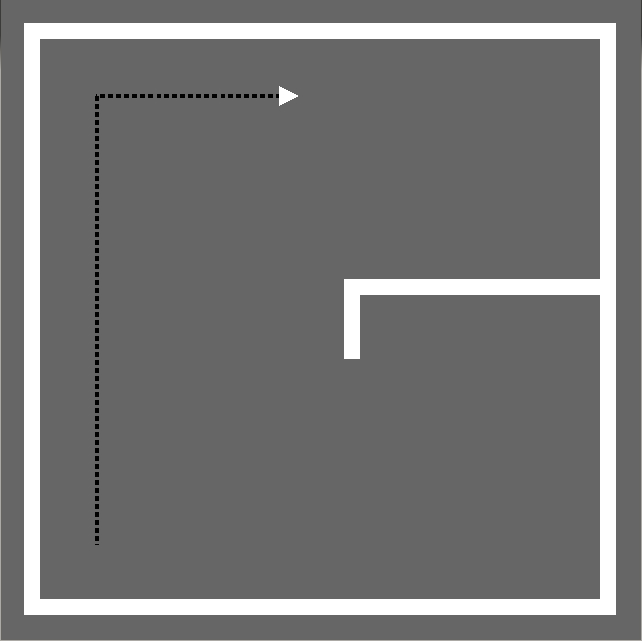
\includegraphics[width=.49\linewidth]{./wall1}
%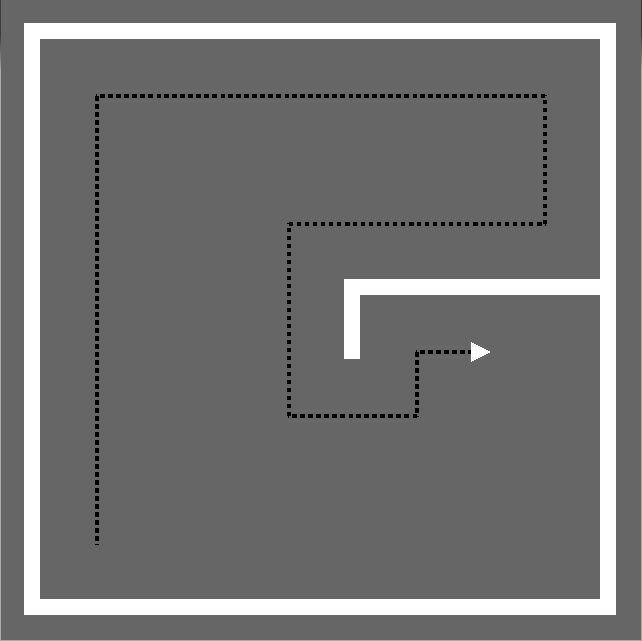
\includegraphics[width=.49\linewidth]{./wall2}
%\caption{Images generated by the robot simulator using the {\tt followWall} program.}
%\label{fig:followwall}
%\end{figure}


%\FloatBarrier
%Set the mood. \docname{} is more of a deep ``Theory'' kind of person 



%Suppose you have just bought yourself a little programmable toy robot
%and you want to design a small DSL in Haskell to program it. The robot
%can turn, move forward and has a sensor to detect whether it is facing
%an obstacle or not. Inspired by the robot language in \cite{} you come
%up with a set of primitives shown in figure
%\ref{fig:interface}. In particular, you would like to use the
%do-notation to sequence programs.

%\begin{figure} 
%\begin{itemize} 
%  \item \verb!move      :: Program ()! 
%  \item \verb!turnLeft  :: Program ()!
%  \item \verb!turnRight :: Program ()!
%  \item \verb!sensor    :: Program Bool!
%  \item \verb!cond      :: Program Bool -> Program () -> Program () -> Program ()!
%  \item \verb!while     :: Program Bool -> Program () -> Program ()!
%  \item \verb!instance Monad Program!
%\end{itemize} 
%\label{fig:interface} 
%\caption{Proposed set of basic robot operations} 
%\end{figure}

%\emph{Example programs}


%The next task is to implement this language. Compiling EDSLs like this
%to something which the physical robot can execute is well know and
%there are off-the-shelf techniques to use. But there is one quirk; how
%does one generate an abstract syntax tree from a type which implements
%the Monad interface?

%Since you want to compile the language there must be an abstract
%syntax tree representation of some sort of the language. The natural
%thing is just to create a new type where each language construct has
%its own constructor. But should you deal with the monadic constructs?
%Well, the simplest solution would be to just add them to the type as well. The resulting type 

%\begin{figure}
%\begin{verbatim}
%data BoolE = Lit Bool
%         | Var String
%         | (:||:) BoolE BoolE
%         | (:&&:)  BoolE BoolE
%         | Not BoolE  

%data Program a where
%  Move      :: Program ()
%  TurnRight :: Program ()
%  TurnLeft  :: Program ()

%  Sensor    :: Program BoolE
%  Cond      :: BoolE -> Program () -> Program () -> Program ()
%  While     :: Program BoolE -> Program () -> Program ()
%   
%  Return    :: a -> Program a 
%  Bind      :: Program a -> (a -> Program b) -> Program b
%\end{verbatim}
%\label{fig:program}
%\caption{A data type for programs}
%\end{figure}

%\emph{More text}

%In the rest of this paper we will see that this na\"ive method
%actually can be made to work and that it's a practical, compositional
%technique for reifying monads.
